\subsection{Caspar}%
\label{sub:caspar}

% Skymaps sind Grundlage einer jeden Datenanalyse
% und sind von besonderem Interesse bei ausgedehnten Quellen,
% oder bei vorhandenseien anderer Quellen im FoV.

Skymaps dienen zur Visualisierung der Messdaten und sind von besonderem
Interesse, um zu überprüfen, ob sich (weitere) Quellen im Blickfeld befinden
oder die Quelle an sich ausgedehnt ist.

\paragraph{Theorie}%

Eine Skymap ist eine zweidimensionale Repräsentation der aufgenommen Ereignisse.
Es gibt drei verschiedene Koordinatensystem, um Ereignisse darzustellen:

\begin{description}
  \item[\quad Kamera Koordinaten] werden genutzt, um die Sensitivität des
    Teleskops
    als eine Funktion in der Kamera zu beschreiben
    (\textit{exposuremap} oder \textit{instrument response function}).
    Eine Repräsentation ist in Abbildung~\ref{fig:cleaning} zu sehen.
    Anhand dieser lassen sich beispielsweise Inhomogenitäten,
    wie sie ein helle Quelle verursacht, bereinigen.
  \item[\quad Azimuthal Koordinaten] sind abhängig von der Position des
    Beobachters auf der Erde.
    Sie sind nicht für die Observation von Astronomischen Objekten von Nutzen,
    aber um die Performance zu testen.
    Dazu werden Daten bei verschiedenen Zenithwinkel verglichen,
    was eine Variation der Atmosphärendicke entspricht.
  \item[\quad Äquatorial Koordinaten] werden genutzt, um eine Skymap einer astrophysikalischen Quelle anzufertigen.
\end{description}

\begin{wrapfigure}{O}{0.36\textwidth}
  \centering
  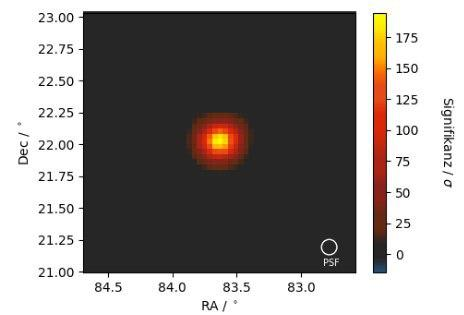
\includegraphics[width=\linewidth]{pictures/skymap.jpg}
  \caption{Skymap einer Beobachtung des Krebsnebels.}%
  \label{fig:skymap}
\end{wrapfigure}

% Die Anfertigung einer Skymap in dieser Analyse ist nicht so simpel wie bei einem gewöhnlichen
% Bild.
Für eine Skymap reicht nicht allein die Konstruktion eines 2D-Arrays,
bei dem die Information allein im Signalverlauf der Pixel enthalten ist,
wie es bei gewöhnlichen Fotos der Fall ist.

Vielmehr wird für jedes Gammaevent ein einzelnes Bild aufgenommen,
auf dem die Richtung rekonstruiert wird.
Eine Skymap bildet eine Menge an rekonstruierten Richtungen im Himmel ab.
Da die Auflösung des Detektors beschränkt ist,
schmieren die rekonstruierten um die wahren Quellposition aus.
Das Ausschmieren der Quelle wird durch die \textit{Point Spread Function (PSF)}
beschrieben
und kann auf einer Skymap bestimmt werden.
Durch die PSF kann das Auflösungsvermögen eines Teleskops
beschrieben werden und bildet daher eine wichtige Größe.

\paragraph{Durchführung}%

Die Konfigurationsdatei \texttt{caspar.rc} wird verwendet.
Es muss das Feld \texttt{Caspar.dataName} angepasst werden.
Wie bei Odie werden die von Melibea prozessierten Daten genutzt.

\begin{lstlisting}
  caspar -q -b --config=caspar.rc
\end{lstlisting}

Caspar erzeugt die Datei \texttt{Output\_caspar.root}.
